\documentclass[mirror, portugues]{revdetua}

% Valid options are:
%   portugues --------- main language is Portuguese
%   final ------------- final version (default)
%   times ------------- use times (postscript) fonts for text
%   mirror ------------ prints a mirror image of the paper (with dvips)
%   visiblelabels ----- \SL, \SN, \SP, \EL, \EN, etc. defined
%   invisiblelabels --- \SL, \SN, \SP, \EL, \EN, etc. not defined (default)
%
% Note: the final version should use the times fonts
% Note: the really final version should also use the mirror option

\usepackage[portuguese]{babel}
\usepackage[utf8]{inputenc}
\usepackage{amsmath} 
\usepackage{comment}
\usepackage{algorithm}
\usepackage{algpseudocode}
\floatname{algorithm}{Algoritmo}
\usepackage{graphicx}
\usepackage[justification=centering]{caption}
\usepackage{float}
\usepackage{booktabs}
\usepackage[table,xcdraw]{xcolor}
%-------------------------------------
% compiling:
% Recipe: xelatex
% Recipe: pdflatex -> bibtex -> pdflatex -> pdflatex
% Recipe: xelatex
%
% notas:
% rever se algoritmos e imagens estão onde devem
%-------------------------------------
\begin{document}

\Header{03}{3}{Janeiro}{2025}{1}

\title{TITULO DO TRABALHO}
\author{Hugo Veríssimo - 124348 - hugoverissimo@ua.pt}
\maketitle

\begin{abstract}
abstrato em ingles
\end{abstract}

\begin{resumo}
abstrato em pt resumo
\end{resumo}


\section{Introdução}

A análise de texto é uma área de estudo fundamental, com diversas aplicações tais como análise de sentimentos ou de opiniões, personalização da experiência do utilizador, recomendação de conteúdo, entre outras \cite{AZ24}. Uma das tarefas centrais nesta área é a identificação da frequência de palavras em grandes volumes de texto, tal como livros, bases de dados ou redes sociais, de modo extrair informações relevantes sobre o conteúdo e estrutura dos textos em análise.

Contudo, a identificação precisa da frequência de palavras em textos de larga escala apresenta desafios significativos, especialmente em termos de memória. Métodos de contagem precisa, que mantêm o registo exato da contagem de cada palavra, revelam-se ineficientes devido ao elevado consumo de memória. Há assim a necessidade do estudo de métodos mais eficientes e escaláveis, principalmente em situações em que os dados estão em constante fluxo, como em \textit{streams} de dados. Neste contexto, algoritmos de contagem aproximada e identificação de itens frequentes têm vindo a ganhar destaque, uma vez que permitem a identificação de palavras mais frequentes de forma eficiente e com uma margem de erro controlada \cite{LH06}.

Este relatório visa explorar três abordagens para este problema: contadores exatos, contadores aproximados e identificação de itens frequentes em \textit{streams} de dados. Para cada uma destas abordagens, será apresentado um algoritmo e .....


%Além da implementação dessas abordagens, será realizada uma análise sobre a eficiência computacional de cada uma delas, considerando o tempo de execução e o uso de memória, bem como suas limitações em termos de precisão e aplicabilidade em diferentes cenários. O objetivo é entender as trade-offs entre precisão e eficiência e fornecer uma base para a escolha do método mais adequado para diferentes tipos de dados e requisitos de processamento. CHATICEGERONIMOPORTUGALTIAGO


\section{Metodologia da Análise}

Para realizar a análise de frequência de palavras, foram selecionados três livros, a partir livraria online \textit{Project Gutenberg} \cite{PG24}, nomeadamente: \textit{Pinocchio: The Tale of a Puppet} (em inglês, EN), \textit{Le avventure di Pinocchio: Storia di un burattino} (em italiano, IT) e \textit{Pinocchion seikkailut: Kertomus marioneteista} (em finlandês, FI). Estes livros foram selecionados por serem traduções do mesmo livro original, conhecido em português como \textit{As Aventuras de Pinóquio}, de Carlo Collodi. A escolha destes livros permite a comparação da frequência de palavras em diferentes idiomas, bem como a análise de semelhanças e diferenças entre as traduções.

Numa primeira fase, os ficheiros de texto descarregados a partir do \textit{Project Gutenberg} foram processados removendo informações irrelevantes, como metadados e licenças, palavras insignificantes e sinais de pontuação. Para além disso todas as palavras foram convertidas para minúsculas e lematizadas. Estas transformações são fundamentais, de modo a simplificar o texto e concentrar a análise nas palavras mais relevantes, garantindo uma avaliação mais precisa e eficiente da frequência de termos. É importante referir que estas transformações foram realizadas com recurso à biblioteca \textit{spaCy}, através do \textit{Python}.


implementar algortimos, analise dos dados, correr ns quantas vezes, .....

numero total de palavras que cada book tem ? n = ?


\section{Contadores Exatos}

Quanto aos contadores exatos, tal como o nome indica, este tipo de técnica é exate, resultando numa contagem precisa da frequência de palavras, no contexto em causa.
O algoritmo apresentado de seguida, designado por \textit{Contador Exato}, é um exemplo de um contador exato, que percorre o texto processado e regista a frequência de cada palavra num dicionário. Este algoritmo é eficiente em termos de precisão, uma vez que mantém um registo exato da contagem de cada palavra, no entanto, revela-se ineficiente em termos de memória, especialmente em situações em que o volume de texto é elevado.

\begin{algorithm}[H]
\raggedright
\textbf{Entrada:} texto processado (\texttt{T}) \\
\textbf{Saída:} dicionário onde as palavras são as chaves e os valores são as suas frequências (\texttt{D})\\
\hrule 
\caption{Contador Exato}
\begin{algorithmic}[1]
    \State \texttt{D} $\gets$ empty dictionary
    \State \texttt{words} $\gets$ list of words from \texttt{T}
    \For{each \texttt{word} in \texttt{words}}
        \If{\texttt{word} $\not\in$ \texttt{D}}
            \State \texttt{D}[\texttt{word}] $\gets$ 0
        \EndIf
        \State \texttt{D}[\texttt{word}] $\gets$ \texttt{D}[\texttt{word}] + $1$
    \EndFor
    \State \Return \texttt{D}
\end{algorithmic}
\end{algorithm}
    
Atendendo à complexidade espacial, no pior caso, onde todas as palavras que constituem o texto \texttt{T} são distintas, a mesma é dada por $O(|\texttt{words}|)$, onde $|\texttt{words}|$ representa o número de palavras no texto. Isto acontece pelo facto do dicionário \texttt{D} conter uma entrada para cada palavra distinta no texto. NAO SEI SE ESTA CERTO, NS SE TENHO DE CONTABILIZAR O TAMANHO DE WORDS AO EM INVES DE SER SO O D ou REFERIR QUE O QUE IMPORTA É O TAMANHO DO DICIONARIO? TALVEZ FALAR DOS DOIS e dps no fim dizer q o words deve ser ignorado pq é o texto e o que importa é o dicionario? idk

comparison of the memory (complexity ?) of the algorithms

.....

através da aplicacao do algoritmo de contagem exata, foi possível identificar as 10 palavras mais frequentes em cada um dos livros analisados. A Tabela \ref{table:top10_exatos} apresenta as palavras mais frequentes em cada idioma, juntamente com o número de ocorrências de cada palavra.

\begin{table}[H]
\centering
\caption{CAPTION top10 palavras mais frequentes em cada idioma}
\label{table:top10_exatos}
\begin{tabular}{lr|lr|lr}
\toprule
\multicolumn{2}{c}{EN} & \multicolumn{2}{c}{IT} & \multicolumn{2}{c}{FI} \\
Palavra & \# & Palavra & \# & Palavra & \# \\
\midrule
pinocchio & 457 & pinocchio & 460 & pinocchio & 443 \\
say & 282 & il & 386 & sanoa & 258 \\
little & 238 & dire & 282 & saada & 143 \\
puppet & 209 & si & 251 & alkaa & 134 \\
come & 141 & burattino & 225 & tehdä & 134 \\
boy & 140 & volere & 167 & marionetti & 131 \\
like & 133 & vedere & 152 & poika & 81 \\
good & 131 & andare & 134 & huutaa & 81 \\
poor & 127 & povero & 134 & nähdä & 80 \\
go & 116 & ragazzo & 126 & kysyä & 77 \\
\bottomrule
\end{tabular}
\end{table}


como seria de esperar, a palavra "pinocchio" é a mais frequente em todos os idiomas, uma vez que se trata do nome do protagonista do livro. Para além disso, é possível observar algumas semelhanças entre os idiomas, nomeadamente a presença de palavras que têm o mesmo siginificado em diferentes idiomas, como "puppet" e "burattino" (marioneta em italiano), ...

para além disso, esta analise tambem permite a analise da quantidade de palavras distintas Fig. \ref{fig:distinc_words} em cada idioma, bem como a distribuição da frequência de palavras Fig. \ref{fig:word_freqs}, o que pode ser útil para a comparação de diferentes traduções de um mesmo livro, por exemplo.

\begin{figure}[H]
    \centering
    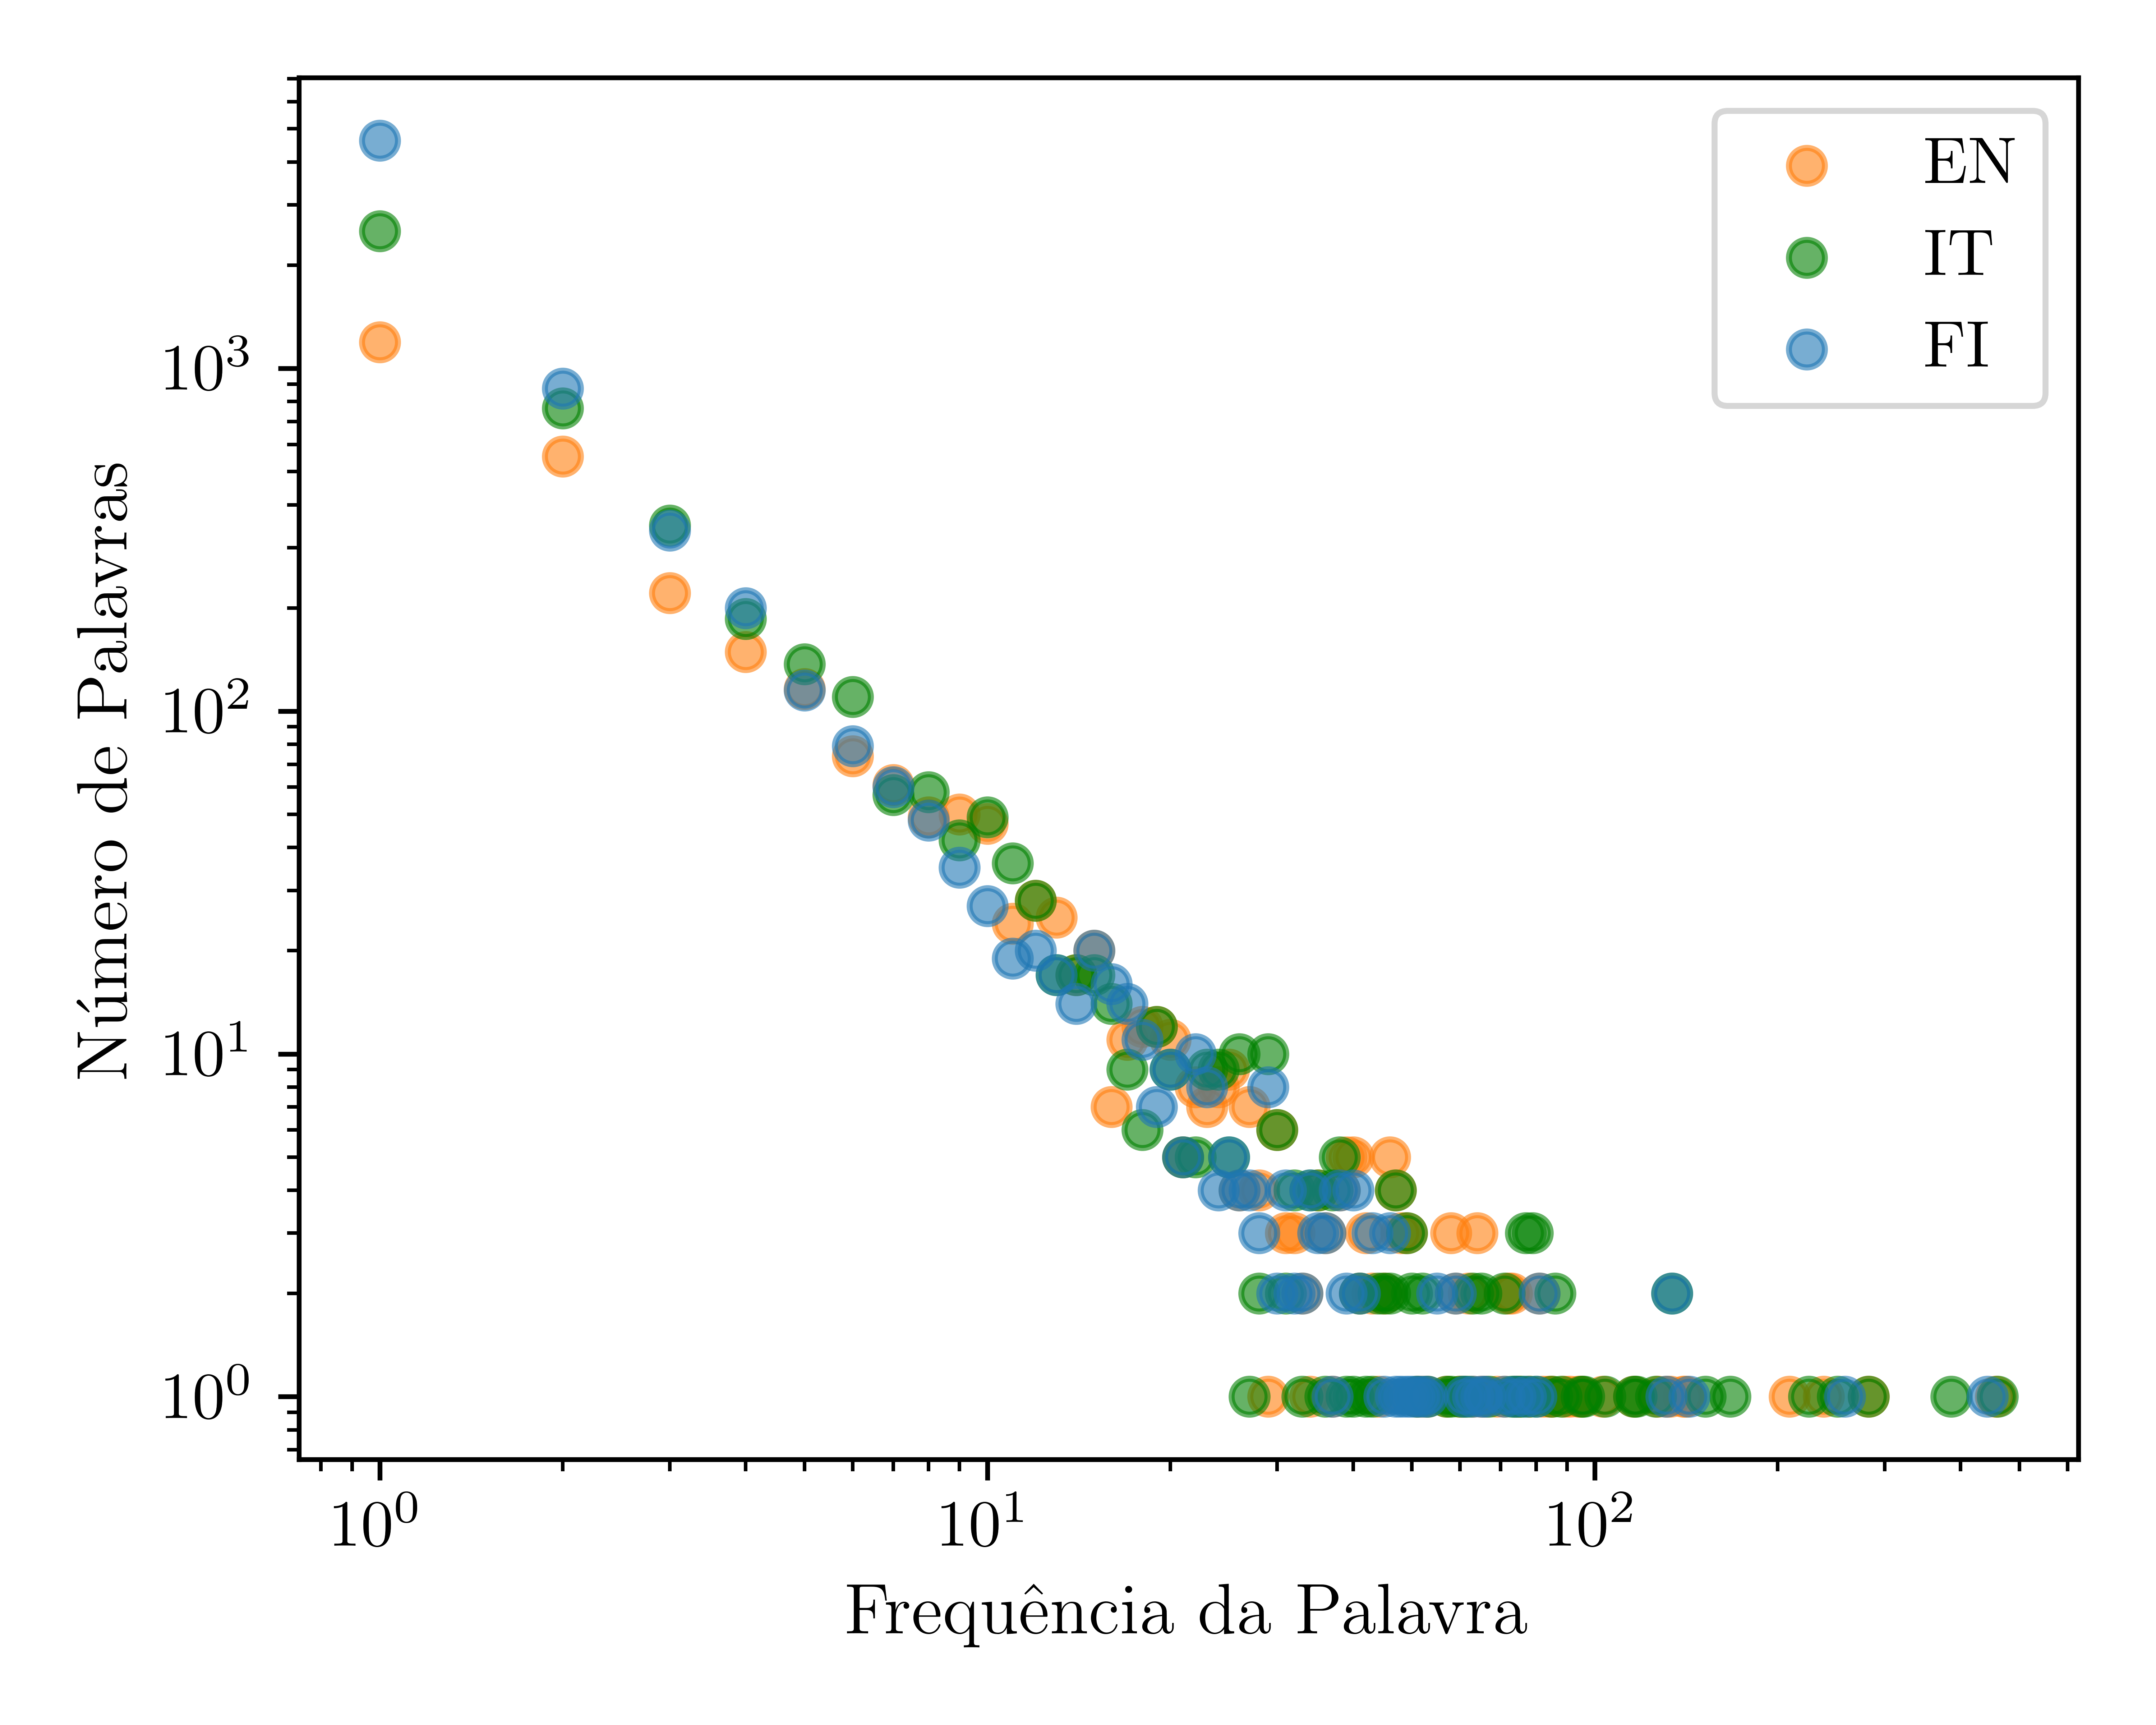
\includegraphics[width=0.45\textwidth]{../assets/exact_word_freqs.png}
    \caption{distribuicao da frequência de palavras em cada idioma}
    \label{fig:word_freqs}
\end{figure}


\begin{figure}[H]
    \centering
    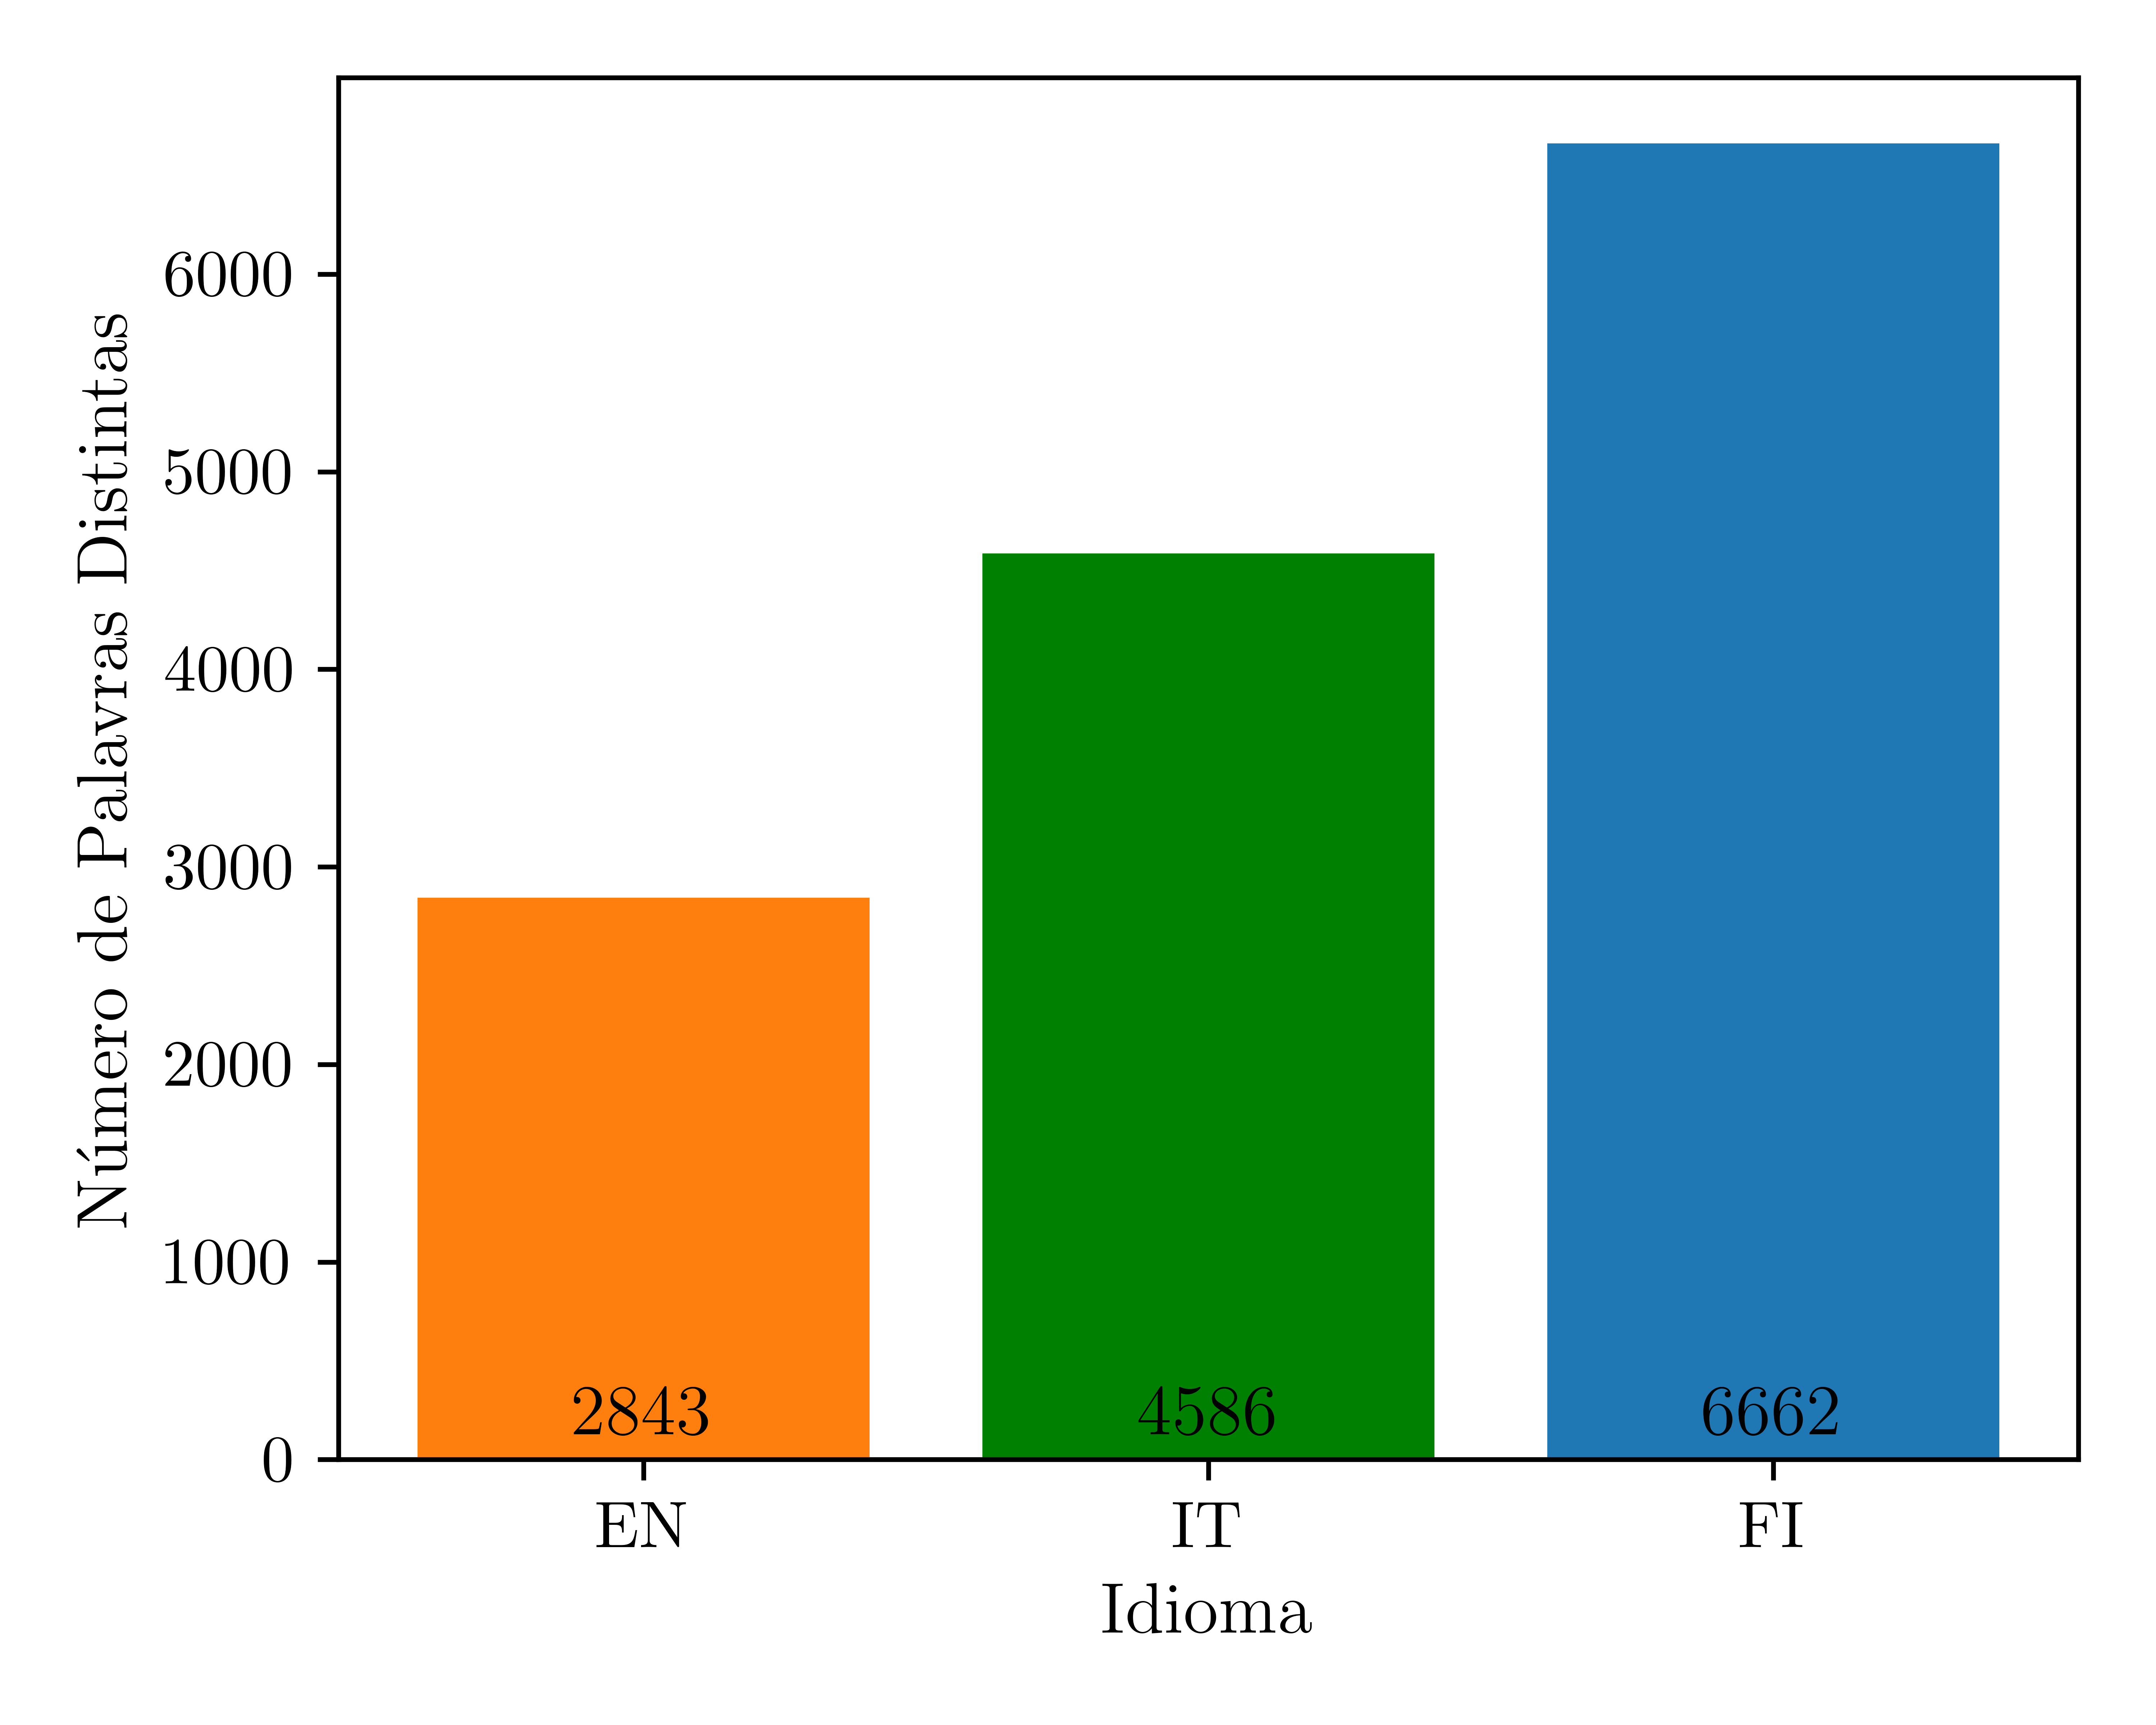
\includegraphics[width=0.45\textwidth]{../assets/exact_distinct_words.png}
    \caption{numero de palavras distintas em cada idioma}
    \label{fig:distinc_words}
\end{figure}

a diferenca pode ter a ver com o desempenho do spacy a lematizar as palavras em diferentes idiomas, ou com a propria complexidade da lingua 






\section{Contadores Aproximados}

Os contadores aproximados, também conhecidos por contadores probabilísticos, inventados por Robert Morris, são algoritmos especializados em realizar estimativas eficientes de contagens, utilizando quantidades reduzidas de memória em comparação com métodos tradicionais, através de técnicas baseadas em probabilidade. Estes contadores são particularmente úteis em situações em que a precisão exata da contagem não é crítica, permitindo uma redução significativa no uso de memória, sem comprometer a qualidade da análise \cite{RM78}.

Um exemplo de um contador aproximado é o algoritmo de contagem aproximada apresentado de seguida, designado por \textit{Contador Aproximado}. Neste exemplo, o algoritmo utiliza uma probabilidade de contagem fixa de $1/16$. Para cada evento, neste caso, cada palavra do texto, é gerado um número aleatório entre 0 e 1, e a palavra é contada se o número gerado for menor que a probabilidade de contagem. Isto permite que a contagem seja realizada de forma aproximada, com uma margem de erro controlada, e um menor uso de memória.

\begin{algorithm}[H]
\raggedright
\textbf{Entrada:} texto processado (\texttt{T}) \\
\textbf{Saída:} dicionário onde as palavras são as chaves e os valores são as suas frequências estimadas (\texttt{D})\\
\hrule 
\caption{Contador Aproximado}
\begin{algorithmic}[1]
    \State \texttt{D} $\gets$ empty dictionary
    \State \texttt{words} $\gets$ list of words from \texttt{T}
    \For{each \texttt{word} in \texttt{words}}
    \State \texttt{r} $\gets$ Uniform(0, 1)
    \If{$r < \frac{1}{16}$}
        \If{\texttt{word} $\not\in$ \texttt{D}}
            \State \texttt{D}[\texttt{word}] $\gets$ 0
        \EndIf
        \State \texttt{D}[\texttt{word}] $\gets$ \texttt{D}[\texttt{word}] + $1$
    \EndIf
    \EndFor
    \For{each \texttt{word} in \texttt{D}} \Comment{Estimate the total count}
    \State \texttt{D}[\texttt{word}] $\gets$ \texttt{D}[\texttt{word}] $\times 16$
    \EndFor
    \State \Return \texttt{D}
\end{algorithmic}
\end{algorithm}

é importante referir q existem outros tipos, diferentes fixed probability, etc.

as contagem sao smp multiplas de 16, pq a probabilidade é 1/16, e dps é multiplicado por 16 para obter a contagem aproximada

complexidade espacial tal tal bla bla

nas tabelas seguintes, por ser um processo aleatorio, apos tere sudo corrido 20 vezes, foi calculada a média, valor max e min de cada palavra, escolhidos as 10 mais frequentes tendo em conta a media, e comparado com a contagem exata. nas tabelas seguintes pode-se observar esses resultados, para cada um dos idiomas analisados. também se repara que as palavras a preto mantiiveram a sua posucao em relacao ao top10 exato, as a laranja estao descoladas mas fazem parte, e as a vermelho não fazem parte do top10 real

\begin{table}[H]
\centering
\caption{top10 dos aproximados sendo o top tendo em conta a media, e media arredondada ao inteiro, e idioma ING}
\label{table:top10_aprox_ingles}
\begin{tabular}{lrrr|r}
\toprule
Palavra & $\text{\#}_{\text{min}}$ & $\text{\#}_{\text{média}}$ & $\text{\#}_{\text{max}}$ & $\text{\#}_{\text{real}}$ \\
\midrule
pinocchio & 336 & 439 & 544 & 457 \\
say & 96 & 270 & 400 & 282 \\
little & 144 & 227 & 320 & 238 \\
puppet & 128 & 223 & 336 & 209 \\
come & 64 & 148 & 240 & 141 \\
boy & 80 & 140 & 176 & 140 \\
\textcolor{orange}{go} & 48 & 132 & 240 & 116 \\
\textcolor{orange}{poor} & 48 & 129 & 240 & 127 \\
\textcolor{orange}{like} & 32 & 128 & 192 & 133 \\
\textcolor{orange}{good} & 64 & 126 & 224 & 131 \\
\bottomrule
\end{tabular}
\end{table}

\begin{table}[H]
\centering
\caption{top10 dos aproximados sendo o top tendo em conta a media, e media arredondada ao inteiro, e idioma italiano}
\label{table:top10_aprox_italiano}
\begin{tabular}{lrrr|r}
\toprule
Palavra & $\text{\#}_{\text{min}}$ & $\text{\#}_{\text{média}}$ & $\text{\#}_{\text{max}}$ & $\text{\#}_{\text{real}}$ \\
\midrule
pinocchio & 240 & 439 & 544 & 460 \\
il & 224 & 379 & 512 & 386 \\
dire & 160 & 263 & 448 & 282 \\
si & 128 & 252 & 320 & 251 \\
burattino & 96 & 223 & 320 & 225 \\
volere & 96 & 169 & 256 & 167 \\
\textcolor{orange}{povero} & 32 & 139 & 240 & 134 \\
\textcolor{red}{bello} & 80 & 133 & 240 & 116 \\
\textcolor{orange}{vedere} & 32 & 131 & 192 & 152 \\
\textcolor{orange}{andare} & 80 & 127 & 192 & 134 \\
\bottomrule
\end{tabular}
\end{table}

\begin{table}[H]
\centering
\caption{top10 dos aproximados sendo o top tendo em conta a media, e media arredondada ao inteiro, e idioma finlandes}
\label{table:top10_aprox_finlandes}
\begin{tabular}{lrrr|r}
\toprule
Palavra & $\text{\#}_{\text{min}}$ & $\text{\#}_{\text{média}}$ & $\text{\#}_{\text{max}}$ & $\text{\#}_{\text{real}}$ \\
\midrule
pinocchio & 320 & 445 & 672 & 443 \\
sanoa & 160 & 266 & 352 & 258 \\
saada & 48 & 160 & 256 & 143 \\
\textcolor{orange}{tehdä} & 48 & 136 & 224 & 134 \\
\textcolor{orange}{marionetti} & 80 & 132 & 224 & 131 \\
\textcolor{orange}{alkaa} & 64 & 104 & 160 & 134 \\
\textcolor{red}{geppetto} & 32 & 87 & 160 & 71 \\
huutaa & 32 & 86 & 128 & 81 \\
\textcolor{red}{pää} & 32 & 80 & 128 & 65 \\
\textcolor{red}{olla} & 16 & 76 & 144 & 61 \\
\bottomrule
\end{tabular}
\end{table}

nota se mais erros quanto menor é a contagem, pq ha maior densidade de palavras, como se viu na contagem exata figura tal


\section{Contadores Space-Saving}

Pelo facto de muitos processos de geração de dados poderem ser modelados como fluxos de dados, que produzem enormes quantidades de informações simples isoladamente, mas que, em conjunto, formam um todo complexo, torna-se interessante a utilização de métodos que respondam rapidamente a cada nova informação e utilizem recursos muito pequenos em comparação com o volume total de dados. Neste contexto, o algoritmo de contagem \textit{Space-Saving} é uma solução eficiente para a identificação de itens frequentes em \textit{streams} de dados, permitindo acompanhar contagens frequentes de forma eficiente, mesmo sob restrições de memória (número máximo de diferentes palavras a manter, $k$) \cite{CG09}.

Este algoritmo é exposto no pseudocódigo seguinte:

\begin{algorithm}[H]
\raggedright
\textbf{Entrada:} \\
- texto processado (\texttt{T}) \\
- número máximo de itens a manter (\texttt{k}) \\
\textbf{Saída:} dicionário com a estimativa das \texttt{k} palavras mais frequentes e respetivas frequências estimadas (\texttt{D}) \\
\hrule 
\caption{Contador \textit{Space-Saving} \cite{CG09}}
\begin{algorithmic}[1]
    \State \texttt{D} $\gets$ empty dictionary
    \State \texttt{words} $\gets$ list of words from \texttt{T}
    \For{each \texttt{word} in \texttt{words}}
        \If{\texttt{word} $\in$ \texttt{D}}
            \State \texttt{D}[\texttt{word}] $\gets$ \texttt{D}[\texttt{word}] + $1$
        \ElsIf{$|\texttt{D}| < \texttt{k}$}
            \State \texttt{D}[\texttt{word}] $\gets$ $1$
        \Else
            \State \texttt{j} $\gets$ $\arg \min_{j \in \texttt{D}}\ \texttt{D}[\texttt{j}]$
            \State \texttt{D}[\texttt{word}] $\gets$ \texttt{D}[\texttt{j}] + $1$
            \State \texttt{D} $\gets$ \texttt{D} $\setminus \{\texttt{j}\}$
        \EndIf
    \EndFor
    \State \Return \texttt{D}
\end{algorithmic}
\end{algorithm}

ao aplicar o algortimo aos dados ...

\begin{table}[H]
\centering
\caption{CAPTION top10 com space saving 10 para os idiomas ingles e finlandes}
\label{table:top10_ss10}
\begin{tabular}{lr|lr}
\toprule
\multicolumn{2}{c}{EN} & \multicolumn{2}{c}{FI} \\
Palavra & \# & Palavra & \# \\
\midrule
boy & 1714 & poja & 1808 \\
time & 1713 & tyytyväinen & 1807 \\
say & 1713 & olinpa & 1807 \\
great & 1713 & sentään & 1807 \\
complacency & 1713 & hullunkurinen & 1807 \\
ridiculous & 1713 & näköinen & 1807 \\
puppet & 1713 & marionetti & 1807 \\
glad & 1713 & onnellinen & 1807 \\
behave & 1713 & muuttua & 1807 \\
little & 1713 & oikeaksi & 1807 \\
\bottomrule
\end{tabular}
\end{table}



quando o k é 10, ve se que todos os valores têm o mesmo valor aproximadamente, o que nao corresponde a realidade, tanto para os resultados dos idiomas apresentados, como para o italiano. isto deve se ao facto de o k ser muito pequeno, e como tal, o algoritmo nao consegue manter a contagem de todas as palavras.


- https://www.vldb.org/pvldb/vol15/p1215-zhao.pdf

- All items whose true count is > n / k are stored ! : n = total number of items, k = number of counters (k = 20 n chega)

- Smallest count min cannot be larger than e x n: IMPLICA AUMENTAR O K ? SIM!!!!

fazer em \% a qnt de k pq é normal ser maior e tal, mas meter o grafico a explicar, posso meter o k = 5 para mostrar os maus resultados e tal e dps meto o grafico e mostro a escolha e tudo mais bla bla

importante dizer q contagens significativas sao aquelas q nao esta tao proximas da media por causa da situacao do n/k +- 1\%

MOSTRAR GRAFICO E DIZER Q OSAO OS PONTINHOS E Q A LINHA É TP OS 10 SIGNIFICATIVOS, O QUE É O MAIS RELEVANTE QUE PQ A ANALISE ESTA MAIORITARIAMENTE FOCADA NO TOP 10

\begin{figure}[H]
    \centering
    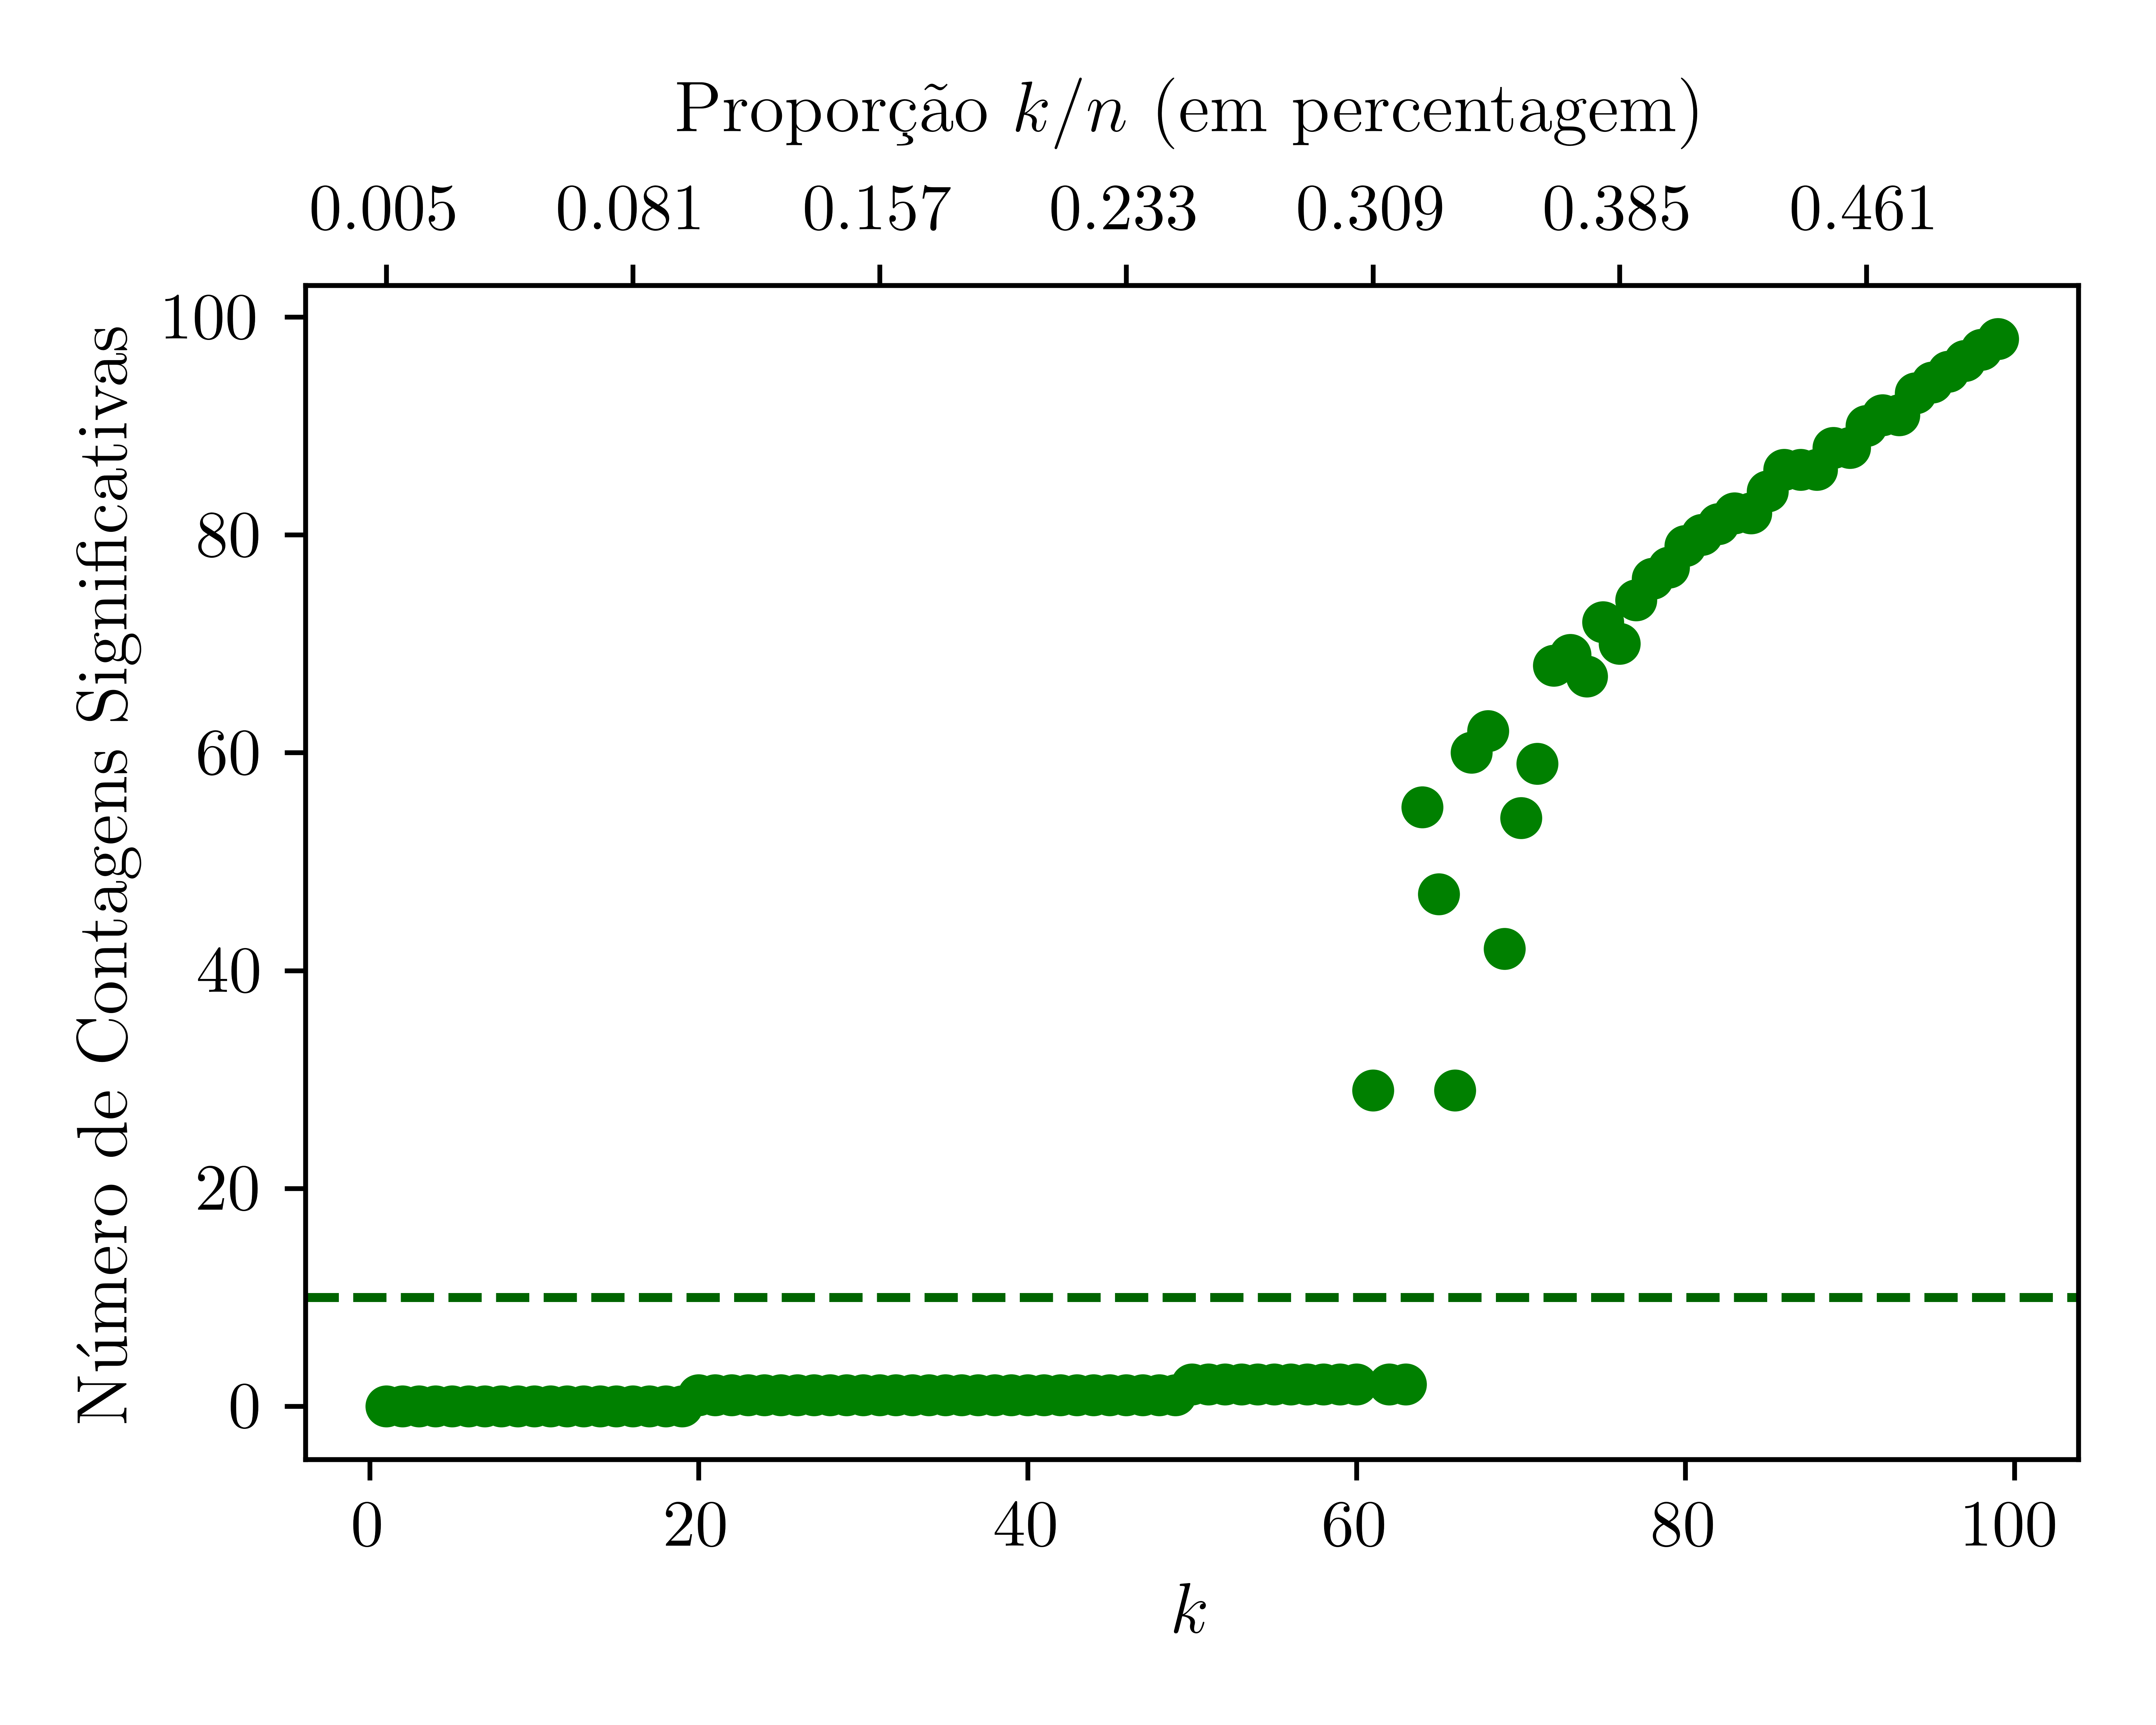
\includegraphics[width=0.45\textwidth]{../assets/ss_signcount.png}
    \caption{qnt de palavras significataivas em funcao de k para o idioma italiano}
    \label{fig:meaningful_wordscount_k}
\end{figure}

falar tbm das percentagens q estao em cima e q, q mostram q o k é bem menor q o numero total de palavras

...

apos analise do valor minimo de k para que haja uma contagem significativa maior que 10, foi observarvado os seguintes valores minimos

\begin{table}[H]
\centering
\caption{CAPTION s}
\label{table:min_k_for_SStop10}
\begin{tabular}{rr|rr|rr}
\toprule
\multicolumn{2}{c}{EN} & \multicolumn{2}{c}{IT} & \multicolumn{2}{c}{FI} \\
$k$ & $k/n$ & $k$ & $k/n$ & $k$ & $k/n$ \\
\midrule
$59$ & $0.344\%$ & $61$ & $0.309\%$ & $67$ & $0.371\%$ \\
\bottomrule
\end{tabular}
\end{table}

como todos os valores, tanto de k sao proximos, de modo a garantir uma certa coerencia ou igualdade ou criterio na comapracao dos resultados, sera aplicado o space savving a todos os livros com k = 70, visto não ser um valor significativo de memoria e ser suficiente para garantir uma contagem significativa de palavras para os 3 livros

para k = 70 temos (falta meter cores e resultado real? SE O TOP10 ESTIVER CERTO, METER COR NA CONTAGEM COM BASE NO DESVIO ABSOLUTO)

\begin{table}[H]
\centering
\caption{CAPTION top10 palavras do SS70}
\label{table:top10_ss70}
\begin{tabular}{lr|lr|lr}
\toprule
\multicolumn{2}{c}{EN} & \multicolumn{2}{c}{IT} & \multicolumn{2}{c}{FI} \\
Palavra & \# & Palavra & \# & Palavra & \# \\
\midrule
pinocchio & 457 & pinocchio & 466 & pinocchio & 443 \\
say & 288 & il & 389 & sanoa & 266 \\
little & 270 & dire & 283 & pieni & 257 \\
good & 244 & burattino & 283 & geppetto & 257 \\
snail & 243 & pesce & 280 & ihmeellinen & 256 \\
fairy & 243 & si & 279 & isä & 256 \\
new & 242 & ragazzo & 279 & vanha & 256 \\
boy & 242 & ciuchino & 279 & istua & 256 \\
look & 242 & geppetto & 278 & pää & 256 \\
geppetto & 242 & fata & 278 & äkkinäinen & 256 \\
\bottomrule
\end{tabular}
\end{table}

os resultados n foram os mlhores, ainda ha confusao ali e talvez paavras nao significativas, pelo que eventualmente podem ser procuradas melhores formas em vez do intervalo em torno da media, mas reparase numa melgoria substancial face ao ss5

assim, de forma empirica, foi selecionado um k = 150

\begin{table}[H]
\centering
\caption{CAPTION top10 palavras do SS150}
\label{table:top10_ss150}
\begin{tabular}{lr|lr|lr}
\toprule
\multicolumn{2}{c}{EN} & \multicolumn{2}{c}{IT} & \multicolumn{2}{c}{FI} \\
Palavra & \# & Palavra & \# & Palavra & \# \\
\midrule
pinocchio & 457 & pinocchio & 461 & pinocchio & 443 \\
say & 284 & il & 386 & sanoa & 261 \\
little & 239 & dire & 282 & saada & 143 \\
puppet & 209 & si & 251 & marionetti & 138 \\
boy & 150 & burattino & 225 & alkaa & 136 \\
come & 145 & volere & 168 & tehdä & 135 \\
good & 135 & vedere & 152 & isä & 128 \\
donkey & 134 & ragazzo & 145 & pieni & 121 \\
like & 133 & bello & 138 & päivä & 119 \\
go & 129 & andare & 137 & pois & 119 \\
\bottomrule
\end{tabular}
\end{table}

observa se uma melhoria substancial nos resultados, principalemnte relativamente ao idioma ingles. idiomas como o finalndes n tiveram uma melhoria tao significativa, mas ainda assim, a contagem é mais precisa e mais proxima da realidade. esta melhoria nao tao significata para a FI deve se a maior quantiade de palavras distintas, o que torna mais dificil a contagem de palavras significativas, mesmo com um k maior e tambem por causa da contagem mais proxima das palavras q estao mais baixo no rank do top 10

isto releva.... (trade off, limitacoes, etc, cada caso, testes de varios k,....)


\section{Resultados}

llalalla

\subsection{analise de memoria}

\begin{table}[H]
\centering
\caption{analise de memoria, em bytes? para cada alg}
\label{table:memoria}
\begin{tabular}{lrrrrr}
\toprule
idioma & Exact & Appro & SS10 & SS70 & SS150 \\
\midrule
EN & 525112 & 359432 & 7984 & 18832 & 33264 \\
IT & 865568 & 572312 & 8064 & 18992 & 33664 \\
FI &1332984 & 884776 & 8176 & 20000 & 35888 \\
\bottomrule
\end{tabular}
\end{table}

\subsection{analise de precisao?}

tendo em conta o rank

\begin{table}[H]
\centering
\caption{ranks top10 para cada alg, em ingles}
\label{table:rank10_ing}
\begin{tabular}{lrrrrr}
\toprule
word & exact & aprox & ss10 & ss70 & ss150 \\
\midrule
pinocchio & 1 & 1 & - & 1 & 1 \\
say & 2 & 2 & 3 & 2 & 2 \\
little & 3 & 3 & 10 & 3 & 3 \\
puppet & 4 & 4 & 7 & 20 & 4 \\
come & 5 & 5 & - & - & 6 \\
boy & 6 & 6 & 1 & 8 & 5 \\
like & 7 & 9 & - & - & 9 \\
good & 8 & 10 & - & 4 & 7 \\
poor & 9 & 8 & - & - & 11 \\
go & 10 & 7 & - & 11 & 10 \\
\bottomrule
\end{tabular}
\end{table}

\begin{table}[H]
\centering
\caption{ranks top10 para cada alg, em italiano}
\label{table:rank10_it}
\begin{tabular}{lrrrrr}
\toprule
word & exact & aprox & ss10 & ss70 & ss150 \\
\midrule
pinocchio & 1 & 1 & - & 1 & 1 \\
il & 2 & 2 & - & 2 & 2 \\
dire & 3 & 3 & - & 3 & 3 \\
si & 4 & 4 & - & 6 & 4 \\
burattino & 5 & 5 & - & 4 & 5 \\
volere & 6 & 6 & - & - & 6 \\
vedere & 7 & 9 & - & - & 7 \\
andare & 8 & 10 & - & - & 10 \\
povero & 9 & 7 & - & - & 12 \\
ragazzo & 10 & 12 & - & 7 & 8 \\
\bottomrule
\end{tabular}
\end{table}


\begin{table}[H]
\centering
\caption{ranks top10 para cada alg, em finlandes}
\label{table:rank10_fi}
\begin{tabular}{lrrrrr}
\toprule
word & exact & aprox & ss10 & ss70 & ss150 \\
\midrule
pinocchio & 1 & 1 & - & 1 & 1 \\
sanoa & 2 & 2 & - & 2 & 2 \\
saada & 3 & 3 & - & 47 & 3 \\
alkaa & 4 & 6 & - & 24 & 5 \\
tehdä & 5 & 4 & - & 25 & 6 \\
marionetti & 6 & 5 & 7 & 19 & 4 \\
poika & 7 & 14 & - & - & 17 \\
huutaa & 8 & 8 & - & - & 135 \\
nähdä & 9 & 12 & - & - & 13 \\
kysyä & 10 & 11 & - & - & 14 \\
\bottomrule
\end{tabular}
\end{table}


- NAO TE PREOCUPES TANTO COM COMPLEXIDADE ESPACIAL, TENS DE TER MAIS EM CONTA OS BYTES... talvez fazer analise de bytes dentro de cada seccao e dps no fim fazer uma tabela 

ou comparacao dos metodos ou assim

- aa - ver erros e isso nos resultados das contagens, de forma quantificada e grafica se der

- analysis of the computational efficiency and limitations of the developed approaches ()

    - absolute and relative errors (lowest value, highest value, average value, etc.)

    - evaluate the quality of estimates

    - same most frequent / less frequent words are identified, and in the same relative order

    - most frequent / less frequent words are similar in the text files of the same book in different language

    - Compare the performance between themselves and regarding the exact counts.

NAS CONTAGENS IGUAIS HA RANKS DIFERENTES, DEVIA METER IGUAL, ACHO Q ISSO SO INTERSSA NA TABELA AGR NA ULTIMA, MAS CONFIRMAR


\section{Conclusão}

conclusaoooo

\bibliography{refs}

\end{document}
